\documentclass{article}
\usepackage[utf8]{inputenc}
\usepackage[english]{babel}
\usepackage{natbib}
\usepackage{graphicx}
\usepackage{authblk}
\title{Business Cycle Transmission between France and United Kingdom}
\author[1]{Blind version}
\affil[1]{University}
\begin{document}

\maketitle

\begin{abstract}
\textbf{Purpose}: The literature mostly investigates the business cycle transmission of UK and France as a part of a wider region (e.g. ERM or G7), despite their historical links and regional significance. Thus, herein paper analyze the interdependence of these economies and how a shock from one of them affects the other for the data since 1978 to 2019.

\textbf{Methodology}: First preliminary statistics were calculated in order to describe the historical relationship between these countries. The econometric part estimates the vector autoregression model to assess the interdependence of the economies. VAR model allows further to inspect the impulse response functions that shows the shock dynamics from one country to another. In order to verify if a shock from one of the economies is important to another, the study uses granger causality test.

\textbf{Findings}: The study establishes a strong link between these countries. A business cycle is transmitted significantly between the economies of France and UK, with a single standard deviation shock from France resulting in a long term effect of $0.4\%$ change in GDP of UK and $1\%$ vice versa. Additionally changes in GDP of both of the countries significantly Granger-cause change to GDP of the corresponding economy.

\textbf{Originality}: This is the first empirical study investigating the business cycle transmission between France and UK and providing a quantitative assessment of their interdependence.

\end{abstract}

\

\textbf{Keywords}: Business cycle, France, UK, England, VAR

\section*{Introduction}

During the great financial crisis in 2008, the world has realized in a painful way how modern economies are interdependent and thus, their economic activity affects each other. Shortly after the Minsky moment of 2008 great financial crisis (GFC hereinafter), which according to many, began in September during a bankruptcy of Lehman Brothers investment bank, the economic contagion quickly spread throughout virtually every country in the world. Even though, the sources of the crisis can be traced to the single sector of handful of advanced economies, the consequences were seen also in countries that by no means had any impact on the processes that led to the crisis. Still this global contagion effect is but a consequence of a globalization, which in overall is a desirable megatrend. After all it is mostly intentional process, shaped by states and international institutions with policies such as liberalization of trade and migratory flows or legislative unification. Given that net benefits of global interdependence are significantly high, there is no urge to change this status quo. That is why it is crucial for economists to understand the mechanics of cross country business cycle transmission, in order to better assess macroeconomic risks and conduct a proper policy rather than eliminate its source. Especially, considering ability of economists to predict incoming recessions or rather lack of thereof \footnote[1]{It is disputable and obviously depend on forecasting horizon. There are papers with robust methods such as \cite{greenwood}, but as reported in \cite{kenny}, in practice forecasting ability is unsatisfying (perhaps due to behavioural reasons, as the forecasters are a subject to animal spirits as well)}

The subject of herein work is even more fundamental. Beginning with the seminal paper of \cite{nelson_plosser}, there is a growing concern among economists about permanent effects of output shocks to economies and thus, that the business cycle is not a simple movement along the trend. Even 10 years after GFC, there is a perception that some countries are still struggling with its consequences or have not done enough with their fiscal policy to curb it (e.g. \cite{IMF} or \cite{house}). Having that in mind, it appears that analysis of international output comovement goes in line with the broader scientific interest.

As chart below shows, the business cycle interdependence measured as standard deviation of GDP across countries included in the World Bank database ($n = 194$) has declined during a period, that globalization was proceeding. Despite the trade wars, global business cycle comovement remains in a downward trend. Even without making any conclusion about relation of both of these phenomena, it is evident, that the mechanism of business cycle transmission is becoming more relevant and likely will continues its trend. 

\begin{figure}[h]
  \centering
  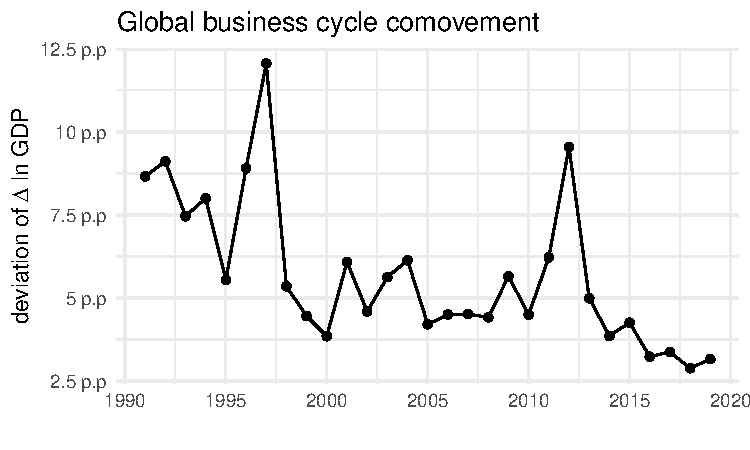
\includegraphics[scale=0.8]{graphs/globalization.pdf}
  \caption{Income comovement trend across 194 countries. Source: World Bank database}
\end{figure}

In order to investigate further the business cycle interdependence, the analysis concerns a pair of developed countries, United Kingdom and France. Both of them are significant for the global economy, thus the result may be considered evergreen across different pairs of countries. These particular countries seems like intuitive pairs to have related business cycle. For most of the historical data, that is subject to empirical part of herein study, both of these countries were members of European Union. Even before its establishment, they perhaps trigger European integration by forming Anglo-French Alliance during treaty of Dunkirk. This long-lasting relationship demonstrate how intense their economic relations are.

Considering a relationship between countries, provides several benefits over an analysis of country-region or region-region business cycle comovement. Primarily, the regional business cycle of European Union is less apparent than the business cycle of its members (\cite{grigoras}). Despite evidence of increasing comovement of real economy (\cite{gogas}) and financial business cycle (\cite{savona}). Therefore, the identification of the transmission can be problematic and sometimes spurious, without providing additional value added to the research. On the other hand, the identification of business cycle of individual countries is free from confounding heterogeneity. Another technical advantage is better data availability due to the shorter existence of regional groups and unions. This directly translates to more robust statistical inference. 

\section*{Literature review}

Before describing actual interdependence on example of France and United Kingdom, it is proper to shed some light on theoretical foundations and empirical findings of business cycle transmission. Channel mechanisms presented in this part are by no means exhaustive, as there is no clear academic consensus on the theory. There are however empirical findings that suggest factors, which could potentially be causal. Although it is hard to distinguish these interested mechanisms from confounders, solely by analysing aggregated macroeconomic data. In general, the business cycle correlation reflects both the nature of the shocks that occurred as well as degree of macroeconomic interdependence. Despite this ambiguity of literature's conclusion, this part of essay will present some explanations of business cycle comovement, particularly by channels such as trade linkages, financial integration and foreign direct investments.

First transmission channel and perhaps the most obvious one is by a trade linkage. This mechanism is related with commonly known empirical relation, that is, country pairs with higher trade with each other also have more correlated business cycle comovement. This empirical regularity was first introduced in a seminal paper of \cite{frankel_rose}, and was confirmed by further studies \footnote[2]{As it is shown later on, the data that is subject to empirical part of this essay, also exhibit such statistical relationship.}. Despite relatively long time of recognition, as well as seemingly high contribution to business cycle transmission of this relation, the theoretical  foundations underlying it, are still ambiguous. Even complex economic models of international real business cycle à la \cite{backus} fail to capture this correlation \footnote[3]{Although, there are recent papers describing IRBC models that allegedly resolve this puzzle such as Ko 2020, but it seems appropriate to await for feedback from scientific community.} \cite{kose}. This issue is especially alarming given large amount of equations in the model and hence, parameters to calibrate in order to obtain satisfying results. Another notable examples of critique in this context is by \cite{imbs}, who points out that country pairs that trade more with each other, tends to have similar economic structure, which implies, that they may be subject to the same sector-specific shocks. All of these questions eventually resulted in a so called trade-comovement puzzle. In theory however, trade linked business cycle transmission may work in a various ways. The most straightforward being a demand-induced channel i.e. negative productivity shock in a single country should decrease its demand for other country products. This channel ought to vary depending on the level of trade between that pair, thus being in line with relationship described by Frankel and Rose.  There is also a more recent paper by di Giovanni et.al 2018, which, based on micro-level data of firms, conclude that sizable effect on business cycle comovement comes from a directly linked large firms. This finding along with the fact that in general there are large inequalities among exporting firms may support the idea of trade as a propagation mechanism. Additionally, such firm-level mechanism is coherent with network effect described by \cite{acemoglu1}, in a way that shock towards a particular firm and hence its output, may result in a contagion of other firms, that are connected to it through a network of input-output linkages. Thus, increasing a scale of the initial shock onto the macro level. This synthesis of works soundly defend the trade related transmission mechanism of business cycle.

Another relevant transmission mechanism is through financial integration. This channel became especially apparent during GFC, when toxic assets were being sold and bought on international markets by financial institutions. Consequently spreading risk to the domestic market, that were hidden at the time. This channel is still relatively poorly described, as the financial sector was not included in the workhorse models of mainstream economists and policy makers before GFC \footnote[4]{There were available models incorporating financial frictions developed in 90s (see e.g. \cite{bernanke_gertler} or \cite{Kiyotaki}}. The main reason for abstract from financial sector was a theorem by \cite{modigliani}, which implies that the funding structure of firms is not important, thus the incorporation of financial sectors in models of a DSGE class may be omitted. However, this theorem was formulated under assumptions of efficient financial markets with perfect information, and as it turned out the asymmetry of the former became crucial in development of GFC.  From an empirical standpoint, there are works suggesting a positive relation between financial integration and business cycle synchronization \cite{imbs}. This relation may be explained in a various ways. Financial markets are commonly place to share risk among market participants with diverse range of instruments. This should lead to smoothing of shocks by distributing given risk among financially integrated countries, thus synchronising their business cycle. This risk-sharing channel is not only achieved with the derivative instruments and others that are meant to hedge against a risk but also with the portfolio exposure to abroad financial factors (e.g. by holding asset-backed securities from USA in 2007). Another channel also observed during GFC is through banking sector. As described by \cite{cetorelli}, this channel spread in a threefold way. First is a decrease in a loan supply from foreign banks, that were subject of the initial shock or were located in a country affected by it. These banks try to curb risk during a stressful time by reallocating funds to safe assets (risk off).  Such foreign bank behaviour also exhibits itself with lower loans supply of their abroad affiliates. Last way of shock transmission is by contraction of domestic loan supply due to the lower activity on international inter-banking market. As it is common in economics, one may find contradictory empirical evidence to even the most common sense idea, and so it is a study by Kalemli-Ozcan and Papaioannou 2009, that provide evidence to the contrary, based on confidential data from bank of international settlements. Their explanations to the negative relation between financial integration and business cycle comovement suggest the reverse causal effect, i.e. that due to the higher benefits from diversification, capital is allocated among country pairs that have different economic structure. In other words, countries that are affected with different shocks (have uncorrelated business cycle) are financially more integrated.  

Another important channel of transmission is through foreign direct investments (henceforth referred to as FDI). As USA data from figure 2 shows, there could be a potential empirical relation between FDI activity and correlation. Except from specific countries like Netherlands, Ireland and Luxembourg, which are known to be subject of multinational tax schemes, the relation between the GDP growth comovement with USA and ratio of FDI stocks to export is positive.

\begin{figure}[ht]
\centering
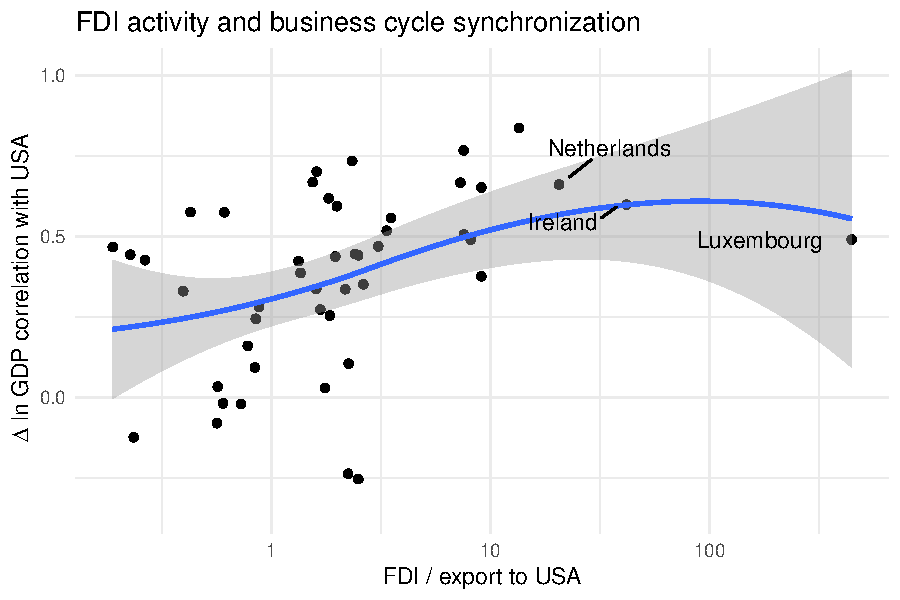
\includegraphics[scale=0.8]{graphs/usa_fdi_plot.pdf}
\caption{FDI activity and production comovement with USA}
\end{figure}

Despite scarcity of data, \cite{jasnen_stokman} also reports from a more statistically rigorous exercise a positive relation between FDI activity and output comovement between given country pairs. Although, their econometric approach may suffer from endogeneity, as they did not control for financial integrity. This variable, according to research described in previous paragraph (\cite{imbs}), is confounding both trade and (theoretically) FDI activity. In spite of allegedly biased estimation of parameters, the direction they reported is most likely true, given the effect size. The FDIs are especially related to the first mentioned channel, i.e. trade, primarily because by reallocating part of the production process to other country (vertical FDI \footnote[5]{Although, the horizontal FDIs are substitutes of trade, thus decreasing it, empirical literature concludes that most of the FDIs are vertical (\cite{carr})}) the investor is ought to transport intermediate goods there, as a part of production chain. The rationale for these kind of FDIs is to save on the difference of factor prices between domestic and foreign market. In this way, the FDI is initiating more trade. This relation is confirmed by data on export and FDI stocks from USA to other countries. The Pearson correlation between their share in GDP in logs is equal to 0.633 \footnote[6]{Own calculation based on data from U.S. Census Bureau, U.S. Department of commerce and World bank.}. This implies, that statistically, the output comovement can be explained by those variables alike. Nevertheless, their theoretical aspects as a transmission channel are interesting in a distinct way. First transmission mechanism is rather straightforward, as economic environment weakens, the owner of FDI abroad is under the pressure to cut employment or even divest entirely to get necessary liquidity. This lead to obvious consequences for country hosting FDI. Another possibility of propagation is through a balance sheet channel. This time the transmission is reversed i.e. if economic conditions decrease in a FDI host country, this will shrink valuation of this project, thus the valuation of investor abroad. Even though it is mostly an accounting event and influence the market capitalization of investor, there is a theoretical nexus linking both of these variables. Lower market capitalization decreases Tobin's Q (\cite{kaldor}), thus changing relation towards replacement value of physical capital and in consequence discourage company to invest. There is also a possible mechanism, that advocates for the common shock hypothesis of business cycle transmission. The FDI, especially from more advanced economies are a source of significant technological spillovers in the hosting economy. This makes economic structure of both of this countries more similar, hence makes them as much vulnerable to the similar shocks. 

The empirical literature concerning particularly the business cycle of France and UK is extremely scarce. Most of the scientific attention is paid to these countries as a part of more regional analysis regarding groups such as ERM (\cite{artis}) or G7 (\cite{fiorito}). There are also some studies comparing their shape of recoveries (\cite{bec}) and sources of business cycle (\cite{karras}).However, to the best knowledge of the author none of the studies tries to analyze the way the business cycle is interdependent between these countries.

\section*{Data and descriptive statistics}


The historical relationship of UK and France is well reflected in their economic data, e.g. on the figure 3. Both times of expansion and downturns are more or less synchronized, sometimes particular time series responds with a lag (visible e.g. in 90s), which will be a rationale for more sophisticated methods employed in a subsequent part of empirical work. Throughout the analysed period, none of these countries were subject to very visible idiosyncratic shocks, whether because of domestic issues or foreign ones. Both of these countries experienced shrinking economies in similar period three times in analyzed period, although periods of expansions were perhaps less synchronized. The crisis at the beginning of 80s had definitively exogenous character. It began with supply shock due to the rising prices of oil. At that time, the dependency on oil of energy markets was similar across countries, thus the reaction was comparable. Next crises had typically for the capitalist economy, an endogenous character, for the shocks that led to them, although deterministic, were a product of chaotic dynamics embedded in economy. That is why their transmission is especially interesting.

\begin{figure}[ht]
\centering
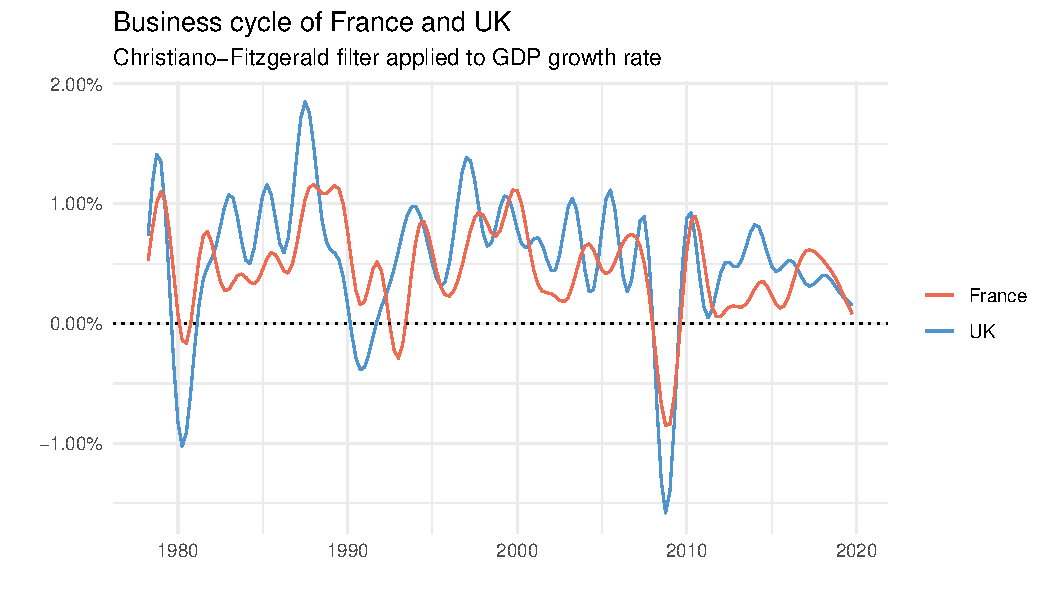
\includegraphics[scale=0.8]{graphs/filtered_cycle.pdf}
\caption{Business cycle of France and UK}
\end{figure}
    
One may come to similar conclusion about their comovement of business cycle from figure 4. There is a supposedly positive relation between quarterly growth of these countries, which is consistent with common sense and economic theory. Both common shock hypothesis and actual business cycle transmission is in line with this relation. Although, the Pearson's correlation is equal only to 0.36. Despite theoretically sound relationship measured, such low correlation coefficient is perhaps because of not controlling for relevant variables and their lags (as figure 3 shows \footnote[7]{If one is accustomed enough with time series analysis, he or she may even notice autocorrelation from figure 4.}).

\begin{figure}[ht]
\centering
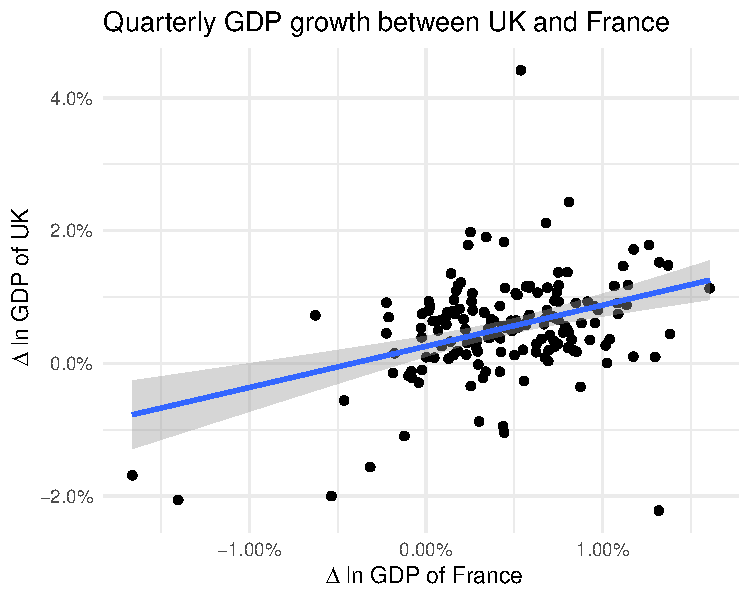
\includegraphics[scale=0.8]{graphs/gdp_fr_uk.pdf}
\caption{GDP growth correlation}
\end{figure}

Despite their close geographical distance, UK nor France are biggest trade partners to each other. France is only 4th direction of UK's export \footnote[8]{According to ONS}, whereas UK is 5th direction of France's export \footnote[9]{ According to Comtrade}. This is obviously still a very close relation and both of their production is dependent on demand from counterparty. With that being said, GDP growth correlation of France with UK is among highest, thanks to, inter alia, their distance and trade relations as is shown on figure 5. 

\begin{figure}[!ht]
\centering
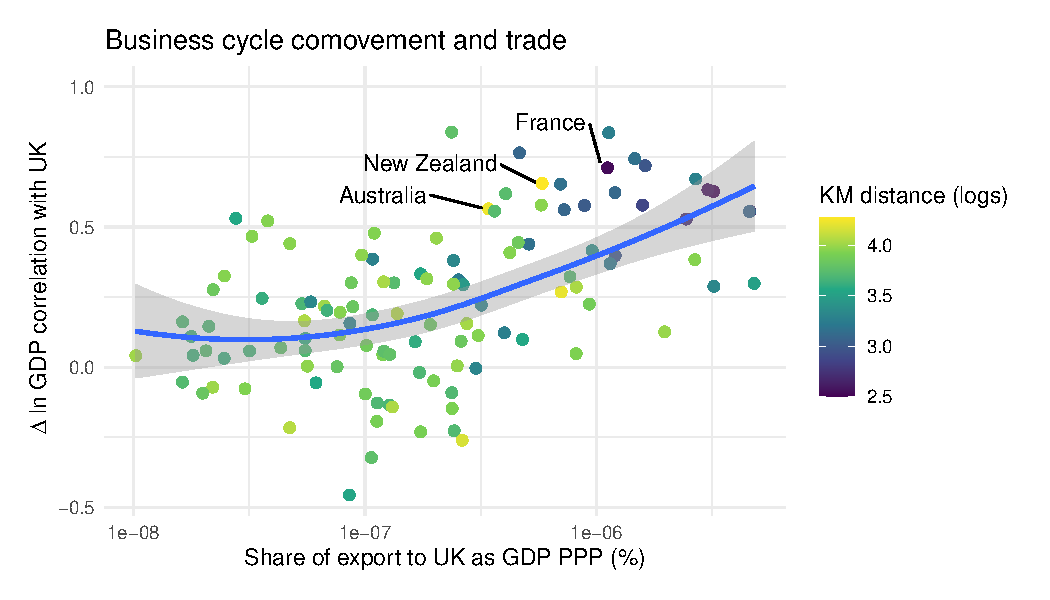
\includegraphics[scale=0.8]{graphs/cross_section_corr2.pdf}
\caption{Income comevement and trade}
\end{figure}

This relation goes in line with the findings of \cite{frankel_rose} of positive relation between trade and business cycle comovement. Certainly, the trade is a function of distance of given partners, thus the trade is a potential confounder of this relationship. However, even after controlling it in a regression such that:

$$ \rho (\Delta Y_uk, \Delta Y_p) = \beta_0 + \beta_1 log_{10}(DIST_{ uk, p}) + \beta_2 log_{10}( EX_{uk, p}) + \epsilon_{uk, p} $$

Where, $\rho (\delta Y_uk, \delta Y_p)$ is a correlation of GDP between UK and other country, $DIST$ is a distance and $EX$ is share of export to UK from partner P. The parameter $\beta_1$ is significant (p-value lower than 0.05), hence indicating that the distance is a valuable variable in itself, i.e. abstaining from trade. Of course the distance per se is not important, but its role as a proxy of unobserved variables such as, similar climate and geographical resources, that often implies similar economic structure of countries. Also cultural similarities of close countries, which explains highlighted position of New Zealand and Australia on the figure 5. As highlighted location of France shows, both the distance and trade with UK is substantial in the context of business cycle comovement, suggesting that modelling their economic relation might prove sensible. 

\section*{Empirical analysis}

As conclusions from previous chapters suggest, there could be a non-trivial statistical relationship between business cycles of these countries. Thus, this chapter describes an approach to modelling this relationship and its outcome. An intuitive approach is to use one of the most popular macroeconometric framework, which is a vector autoregression model (VAR hereinafter) as described in \cite{sims}. In general a VAR model is a n-equation linear regression model with n-variable, each explained by its own lagged values and lagged values of other variables. Given its atheoretical constructions, it is suitable for modelling phenomena, which theoretical foundations are ambiguous, as described in second chapter. Additionally, VAR framework provides several tools that will be also utilized in this chapter.

A small linear vector autoregression model is used with 2 endogenous and 4 exogenous variables. The data is a quarterly time series with macroeconomic variables ranging from 1978Q1 to 2019Q3, gathered from Eurostat and OECD data, then pre-processed. 

A general assumption regarding time series data in econometric modelling is its stationarity. Formally speaking this means, that a vector $x_t$ have time-invariant first and second moments i.e. $E[x | t] = \mu$ and $\mathcal{V}[x | t] = \sigma^2$. Most of the variables are non-stationary in levels but after transforming variables with first difference  or logarithms, each shows stationarity according to test developed by \cite{perron}. The lag order of VAR model was chosen according to Akaike-Information Criterion (\cite{Akaike1998}) and was estimated with a standard OLS method giving following system of data-generating process:


$$\Delta ln Y_{uk, t} = \beta_0 + \beta_1 \Delta ln Y_{uk, t-1} + \beta_2 \Delta ln Y_{fr, t-1} + \beta_3 \Delta ln FX_t + \beta_4 \Delta r_{uk, t} + \beta_5 \Delta \pi_{uk, t} + \epsilon_t$$

$$\Delta ln Y_{fr, t} = \theta_0 + \theta_1 \Delta ln Y_{fr, t-1} + \theta_2 \Delta ln Y_{uk, t-1} + \theta_3 \Delta ln FX_t + \theta_4 \Delta r_{fr, t} + \theta_5 \Delta \pi_{fr, t} + \gamma_t$$

Where, $\beta$ and $\theta$ are variable parameters for equations of respectively, United kingdom ($uk$) and France ($fr$). $Y_{t}$ is a vector of  real GDP, $FX_t$ is an exchange rate between currencies of these countries. $r_t$ and $\pi_t$ are respectively short term (less than 24h) interbank rate and consumer price index. $\epsilon_t$ and $\gamma_t$ are error terms. Estimated parameters of the model are shown in the table below.

\begin{table}[ht]
    \centering
    \begin{tabular}{rrrrr}
      \hline
     & Estimate & Std. Error & t value & Pr($>$$|$t$|$) \\ 
      \hline
    $\Delta ln Y_{uk, t-1}$ & 0.1254 & 0.0809 & 1.55 & 0.1230 \\ 
    $\Delta ln Y_{fr, t-1}$ & 0.4302 & 0.1313 & 3.28 & 0.0013 \\ 
      $\beta_0$ & 0.0049 & 0.0010 & 4.79 & 0.0000 \\ 
    $\Delta ln FX_t$ & -0.0179 & 0.0179 & -1.00 & 0.3207 \\ 
    $\Delta r_{uk, t}$ & -0.0004 & 0.0006 & -0.74 & 0.4621 \\ 
    $\Delta \pi_{uk, t}$ & -0.0042 & 0.0011 & -3.71 & 0.0003 \\ 
       \hline
    \end{tabular}
    \end{table}
    
    \begin{table}[ht]
    \centering
    \begin{tabular}{rrrrr}
      \hline
     & Estimate & Std. Error & t value & Pr($>$$|$t$|$) \\ 
      \hline
    $\Delta ln Y_{uk, t-1}$ & 0.1720 & 0.0402 & 4.28 & 0.0000 \\ 
    $\Delta ln Y_{fr, t-1}$ & 0.4266 & 0.0670 & 6.37 & 0.0000 \\ 
    $\theta_0$ & 0.0019 & 0.0005 & 3.83 & 0.0002 \\ 
    $\Delta ln FX_t$ & -0.0137 & 0.0091 & -1.51 & 0.1330 \\ 
    $\Delta r_{fr, t}$ & 0.0006 & 0.0003 & 2.04 & 0.0429 \\ 
    $\Delta \pi_{fr, t}$  & -0.0006 & 0.0007 & -0.82 & 0.4151 \\ 
       \hline
    \end{tabular}
    \end{table}


Estimated VAR model meets assumptions that are specific to the vector autoregression model, such as parameter stability, as well as assumptions of OLS of strict exogeneity, lack of perfect multicollinearity and error autocorrelation. The innovation process satisfy proper assumptions such as $E[\epsilon_t] = 0$, $E[\epsilon_t \epsilon_s '] = 0, s \neq t$ (no serial correlation among error terms) and $E[\epsilon_t \epsilon_t '] = \Sigma$ (covariance matrix of error terms is positive-semidefinite). Some of the parameters are insignificant, however, they are used merely as a control variable and won't be a subject of statistical inference standalone. Even though, the model is diagnosed based on in-sample data, it fits very well, given the complexity of actual economic mechanism. 


With estimated VAR model, it is now possible to inspect how UK business cycle is transmitted to France and vice versa. In order to do that the impulse response functions (IRF) were estimated with simulations of system of equations described earlier. These function shows how shock to a given equation affect the other, which we assume represents the transmission of business cycle. Mathematically it is a single standard deviation shock to $\epsilon_t$ or $\gamma_t$ into our system of equations and reaction from endogenous variable $\Delta ln Y_{t}$ for $fr$ and $uk$. The bootstrapping of the IRF along with corresponding confidence $95\%$ intervals was executed with 10 000 runs. Following figures shows path of the estimated IRFs:

\begin{figure}[!ht]
\centering
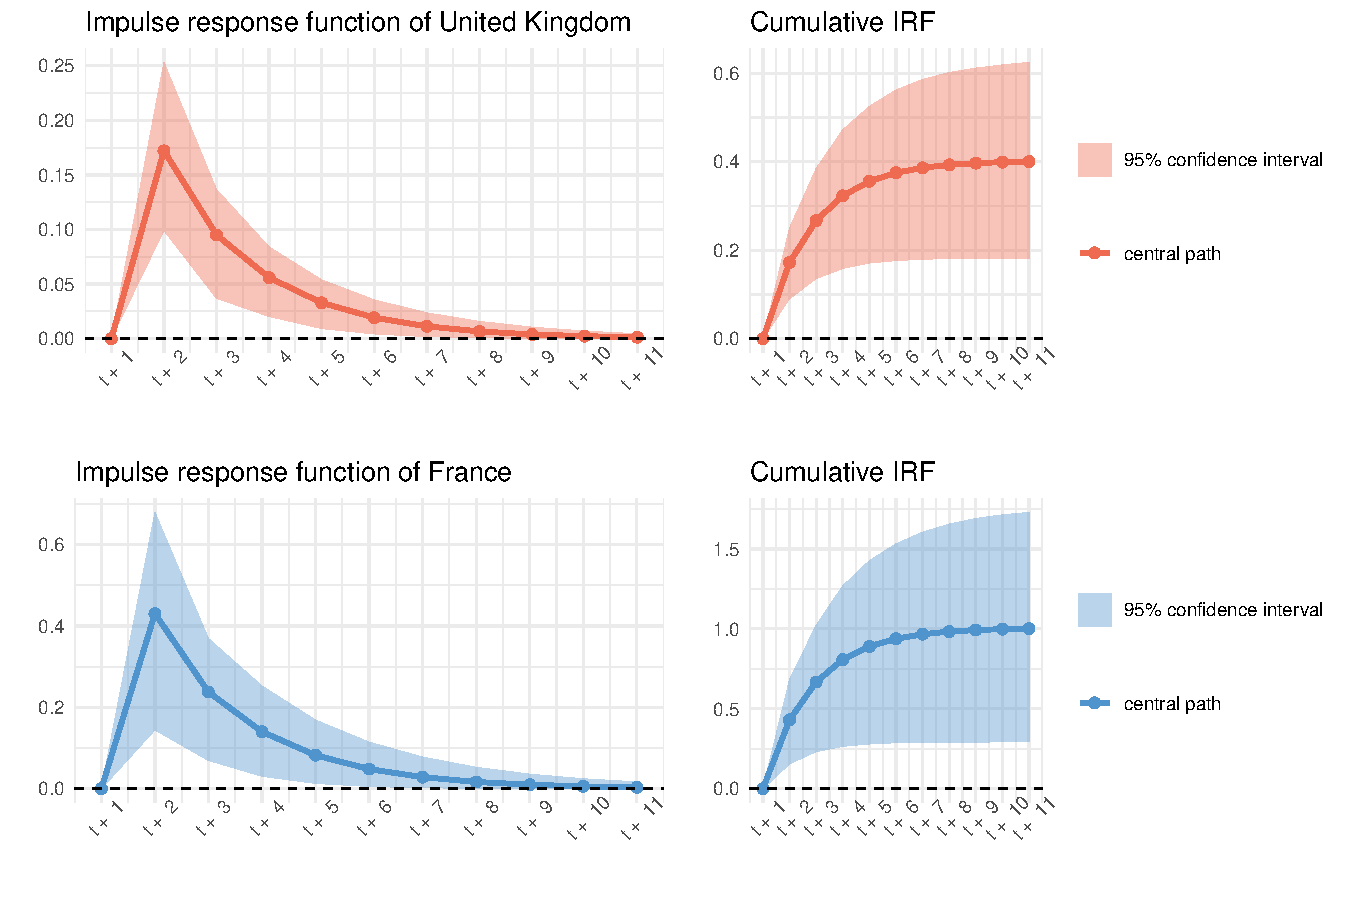
\includegraphics[scale=0.6]{graphs/irf_plot.pdf}
\caption{Impulse response functions}
\end{figure}

A natural question arises of the causality. With the research design applied, it is insightful to determine the granger-defined causality (\cite{granger}), which states that if a lagged variable $X_{t-1}$ contains enough information in order to significantly predict variable $Y_t$, then it is assumed that it granger cause it. Mathematically, it is a simple F-test performed on coefficients of bivariate VARs. The hypotheses of Granger test are following:

\

$H_{uk}0$: $\Delta ln Y_{uk}$ do not Granger-cause $\Delta ln Y_{fr}$

and

$H_{fr}0$: $\Delta ln Y_{fr}$ do not Granger-cause $\Delta ln Y_{uk}$

\

Both of the hypotheses fail with p-value of respectively $0.001095$ and $0.002$. This means that shock in the production of UK economy granger cause shock in the economy of France and vice versa. Both of the business cycles are affected by each other, which implies that these countries exhibit a so called feedback loop, meaning that a shock from a given country comes back, albeit, with a gradually decreasing impact. This feedback loop is also shown on the IRF as the simulations used to estimate them are stochastic processes generated from the whole system of equations, that depend on each other.

\section*{Results}

The economic activity is evidently transmitted between these countries. The function of both of the equations is significantly higher than 0. The positive shock in a given country results in a positive shock to another. The effect is highest for both countries at time $t_2$ and then gradually decreases until $t_7$ for UK and $t_6$ for France. The magnitude of the response is higher for France than UK, which could be explained by a difference of GDP among these countries.

The productivity shock from both of these countries have a lasting effect on the other one, with timespan of around 6 quarters. Yet, the two countries differ in the sensitivity and channels of transmission. Because of the sheer size of UK's economy, the impact it make to the France is higher as seen on the Figure 6. (especially the cumulative IRF). On the other hand, since the UK's economy is more dependent on rest of the world when comparing to France, the size of impact is lower. Although, still not negligible and having similar lifespan. 

As the estimated parameters suggest, the two economies react to different variables as well. Despite having much lower impact, the variables also important to the model are short term rates and inflation. However, in the context of business cycle transmission only the inflation is  worth the attention given the effect size. Which is sensible as the inflation shows the current level of overheating in the economy.

At least in this model specification, the exchange rate cannot be distinguished as a particularly significant channel of business cycle transmission. This may be due to the euro being common currency to third countries outside of countries subject to the research. Thus, hiding the representativeness of French economy in the euro exchange rate dynamics. 

Overall, the model shows that real economy, unlike the financial part of it (including exchange rates) is the most dominant channel of business cycle transmission. This is mostly because of very deep market integration and free trade agreement between them. 

\section*{Conclusion}

Herein study demonstrated business cycle transmission between UK and France in the view of theoretical foundations as well as empirical findings from previous studies. The empirical part of the analysis presented econometric modelling of business cycle of UK and France. It is evident that economies of these countries are related. For both countries, after controlling for other variables, a shock in given economy resulted in shock in corresponding economy. This result is in accordance with literature and theory. However, this approach is still not sufficient to identify causal links between these countries. The alternative explanation, that is consistent with the common shock hypothesis is that the economic structure of UK and France is similar, thus responds in a similar way but merely with different time of the response. It is indeed hard to argue that these countries are not similar. Both were for a long period of analyzed data in UE or other close union and their cultural heritage comes from similar roots. With that being said, the evidence to the contrary is still rather dominating. Theoretical studies lacks sound explanations regarding the lagged reaction to common shock of some countries. If an economic structure is indeed similar, then the reaction to the common shock should as well be in the same time. 


Despite limited insight regarding causal links or accurate description of microfoundations of the underlying phenomena, there is indeed a value added from herein research. First and foremost, the modelling provides a statistically sound and quantitative description of relationship between those countries, thus assessing macroeconomic risk that both of these countries bear, in case of shock from abroad. This is the most practical insight for macroeconomics risk management, that may even abstract from the underlying mechanism. As noted in the introduction, the globalization that most likely leads to the business cycle synchronization is a megatrend that won't be reversed all of sudden, thus assessing the impact of shocks from abroad is essential to conduct a proper policy. 

\section*{Supplementary data}

Data pre-processing, visualization and statistical modelling was done in R language. Script with code for reproduction of data analysis may be found on author's repository: (this is deleted for the purpose of blind review). Sources of the data come from following sources: Eurostat, OECD, ONS, Worldbank, USA census.


\bibliography{bibliography}
\bibliographystyle{apalike}

\end{document}



